\documentclass[a4paper, oneside]{book}

\usepackage{amsmath, systeme, amsfonts}

\DeclareMathOperator*{\argmax}{arg\,max}
\DeclareMathOperator*{\argmin}{arg\,min}

% -- Настройка боковых заметок ------------------------------------------------
\usepackage[a4paper, marginparwidth=6cm, marginparsep=0.8cm]{geometry}
\geometry{left=1.5cm}
\geometry{right=8cm}

\setlength{\marginparpush}{15pt}


\usepackage[T2A]{fontenc} % Use 8-bit encoding that has 256 glyphs
\usepackage[utf8]{inputenc} % Required for including letters with accents
\usepackage[russian]{babel}
\usepackage{graphicx}

% marginnote создает НЕ нумерованные плавающие боковые заметки
\usepackage{marginnote}

% Здесь делаем маленький шрифт для marginnote
\let\oldmarginpar\marginpar
\renewcommand\marginpar[1]{\-\oldmarginpar[\raggedleft\footnotesize #1]%
{\raggedright\footnotesize #1}}

% sidenotes создает НУМЕРОВАННЫЕ плавающие боковые заметки и боковые картинки
\usepackage{sidenotes}
% Здесь делаем маленький шрифт для sidenotes
\makeatletter
\RenewDocumentCommand\sidenotetext{ o o +m }{%      
    \IfNoValueOrEmptyTF{#1}{%
        \@sidenotes@placemarginal{#2}{\textsuperscript{\thesidenote}{}~\footnotesize#3}%
        \refstepcounter{sidenote}%
    }{%
        \@sidenotes@placemarginal{#2}{\textsuperscript{#1}~#3}%
    }%
}
\makeatother
% -----------------------------------------------------------------------------

% -- Настройка библиографии ---------------------------------------------------
\usepackage[backend=biber]{biblatex}
\addbibresource{biblio.bib}
% -----------------------------------------------------------------------------

% % -- Настройка форматирование глав и секций -----------------------------------
% \usepackage{titlesec}
% 
% \titleformat
% {\chapter} % command
% [display] % shape
% {\bfseries\Large\itshape} % format
% {Story No. \ \thechapter} % label
% {0.5ex} % sep
% {
%     \rule{\textwidth}{1pt}
%     \vspace{1ex}
%     \centering
% } % before-code
% [
% \vspace{-0.5ex}%
% \rule{\textwidth}{0.3pt}
% ] % after-code
% 
% 
% \titleformat{\section}[wrap]
% {\normalfont\bfseries}
% {\thesection.}{0.5em}{}
% 
% \titlespacing{\section}{12pc}{1.5ex plus .1ex minus .2ex}{1pc}
% % -----------------------------------------------------------------------------

\usepackage[breaklinks,hidelinks]{hyperref}


\title{Конечные структуры \\ {\Huge в примерах}} % The article title

\author{Садыков Нурлан}

% Абстракт
% Заметки по решению кубика рубика с помощью теории групп.

\begin{document}

\maketitle  
\chapter{Кубик Рубика}
\section{Где здесь группа?}


\begin{marginfigure}
    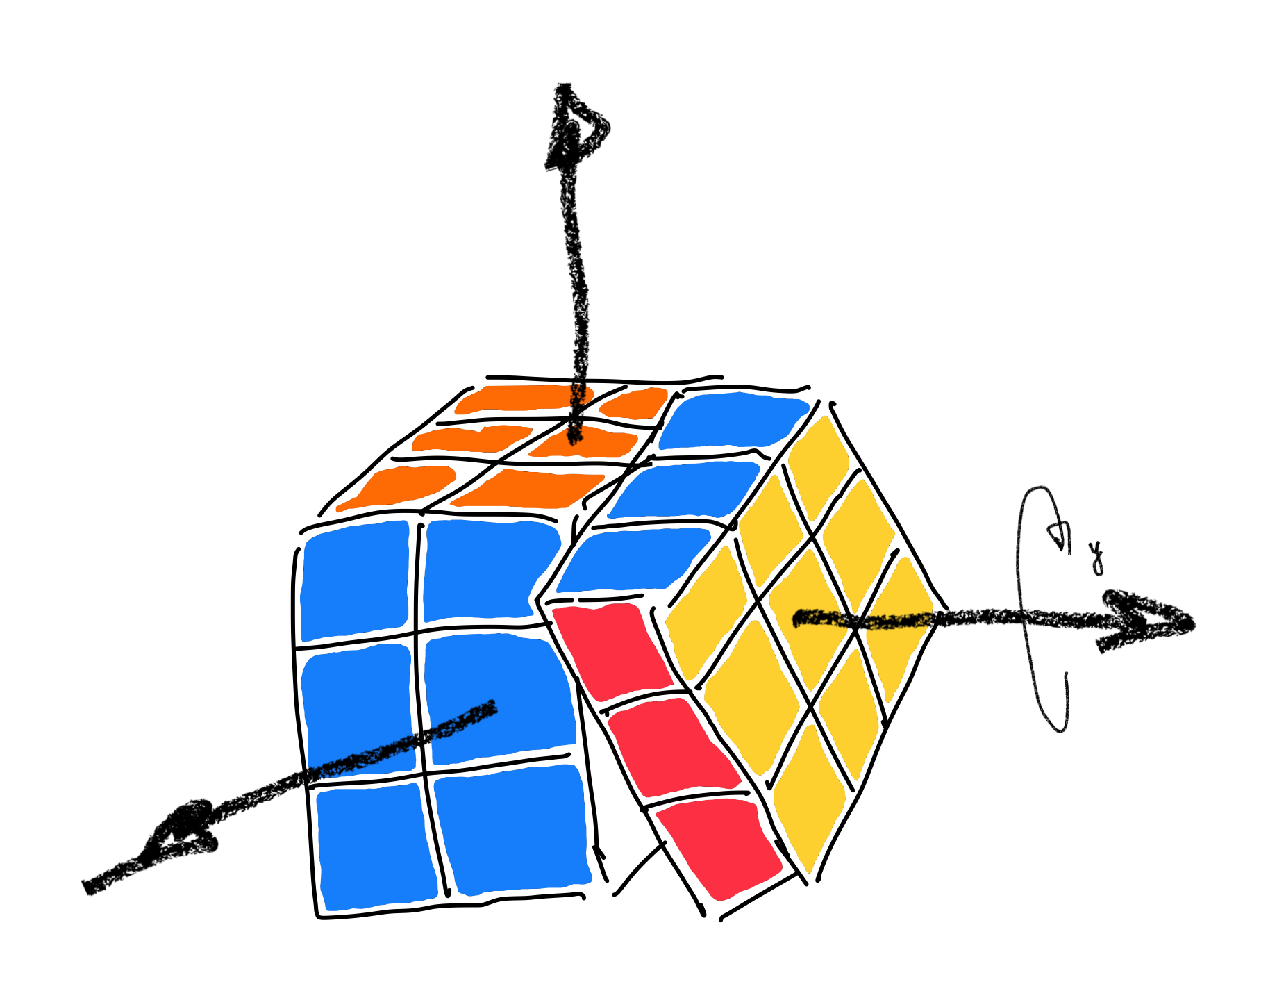
\includegraphics[width=1.1\columnwidth]{../pics/rubik_single_move.pdf}
    \caption{Движение желтой грани $y$}
    \label{fig:move_y}
    %\setfloatalignment{b}
\end{marginfigure}


Обозначим вращения граней кубика\marginpar{
    Под вращением грани понимаем ее поворот на $90^\circ$ по часовой стрелке
    относительно остальной части кубика.
} в соответствии с
цветом центрального стикера на грани. Это удобно потому, что вращения граней
всегда оставляют центральные стикеры на месте. Будем обозначать эти вращения
цветами соответствующих граней: $o$-оранжевый, $b$-синий, $r$-красный,
$y$-желтый, $w$-белый, $g$-зеленый. Вращения граней кубика рубика являются
образующими свободной группы. Любое слово в этой группе можно применить как
инструкцию к кубику рубика. Будем считать слово тривиальным, если после его
применения к собранному кубику, мы снова получим собранный
кубик.\marginpar{Любые промежуточные состояния применения слова к кубику не
обязаны давать собранный вариант.} Например, очевидно, что $b^4 = bbbb = e$ то
есть вращение относительно синей грани четыре раза --- тривиальное слово,
поскольку снова дает правильную сборку.

Для определенности будем считать, что мы применяем слова к кубику слева
направо. То есть слово $oby$ это сперва повернуть оранжевую грань на
$90^\circ$, потом синюю и только потом желтую.

\section{Кодировка состояния кубика}
\begin{marginfigure}
    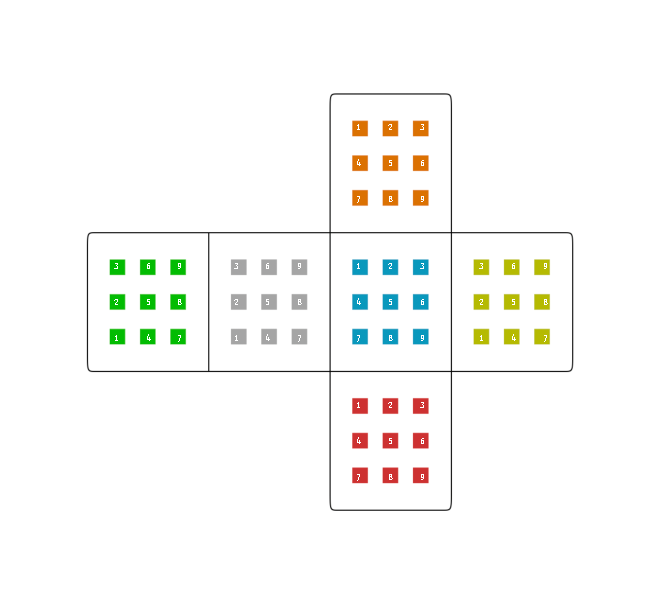
\includegraphics[width=1.1\columnwidth]{../pics/rubik_index_involute.pdf}
    \caption{Индексация стикеров на развертке}
    \label{fig:indexes}
    %\setfloatalignment{b}
\end{marginfigure}

Каждое действие переставляет стикеры на кубике Рубика, значит группа действий
на кубике может быть описана как подгруппа группы перестановок. Чтобы явно
определить перестановку по какому-либо состоянию нужно ввести
кодировку.

Для удобства мы будем обозначать элементы цветом и индексом, например, $b_5$
будет обозначать центральный синий стиркер. Индексы на каждой грани
определяются в соответствии с рисунком~\ref{fig:indexes}.

Как только мы ввели кодировку, можем проследить какой стикер стоит на какой позиции. И уже отсюда можем вытащить перестановки.

\subsection{Неполная кодировка} 

Если цветам приписать такие векторы
$o=(0,\,0,\,1)$, $b=(1,\,0,\,0)$, $y=(0,\,1,\,0)$, $w=(0,\,-1,0)$,
$g=(-1,\,0,\,0)$, $r=(0,\,0,\,-1)$, то можно определить начальную координату
каждого маленького кубика в кубике Рубика как сумму цветов входящих в маленький
кубик. Так можно было ввести кодировку состояния кубика Рубика, но она
получится неполной. Чтобы убедиться в этом достаточно посмотреть на слово
$\alpha = oywgbrowygbr$. Если его применить к начальному состоянию, вершинная
кодировка покажет тривиальную перестановку, но мы не получим начальное
состояние. Так происходит потому, что это слово меняет ориентацию некоторых
кубов на границах двух цветов. Слово $\alpha^2=e$ уже будет тривиальным.

\begin{marginfigure}
    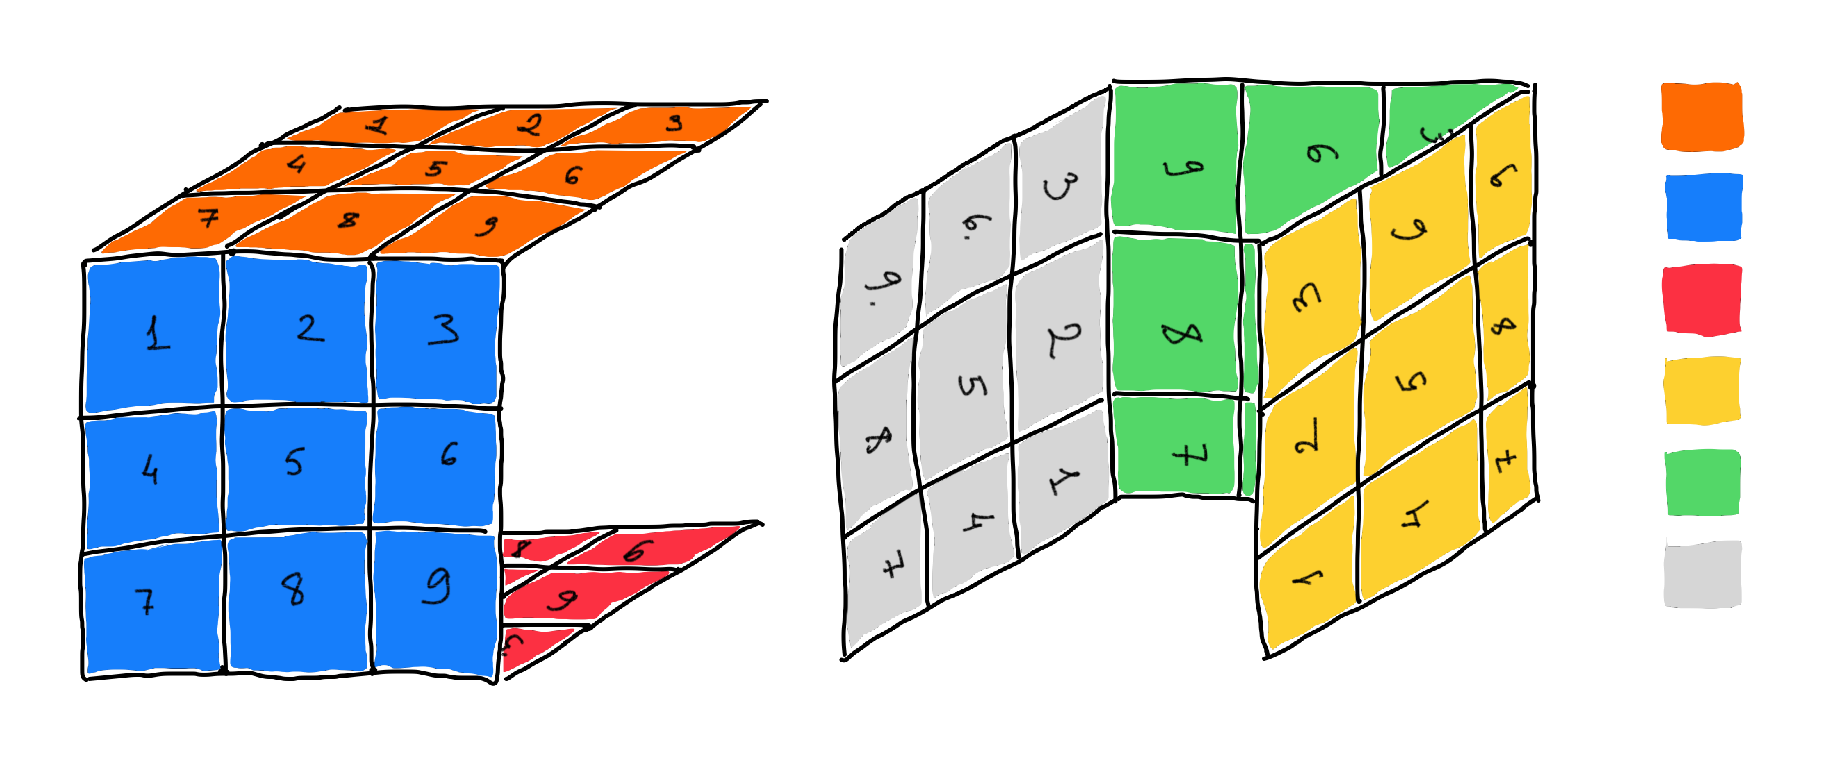
\includegraphics[width=1.1\columnwidth]{../pics/rubik_prepresentation.pdf}
    \caption{Разрез кубика на две ленты с нумерациями.}
    \label{fig:representation}
    %\setfloatalignment{b}
\end{marginfigure}

Неполную перестановку можно использовать, чтобы упростить задачу поиска разложения на слова. Поскольку эта группа содержит всего 20 элементов некоторые задачи можно будет решить перебором.

\paragraph{3-циклы}
Можно найти представления в виде слов всех 3-циклов в неполной кодировке. Схема
поиска следующая. 

\marginpar{
    \emph{Трюк 1:} Разложение цикла в произведение пермутаций \[
        (a_0\; a_1\; a_2\; \cdots\; a_k) = (a_0\; a_1)\,(a_0\;a_2)\,\cdots\,(a_0\;a_k)
    \]
}

\marginpar{
    \emph{Трюк 2:} Объединение двух не коммутриющих пермутаций в 3-цикл \[(a\; b)\, (a\; c)  = (a\; b\; c)\]
}

\marginpar{
    \emph{Трюк 3:} Объединение двух коммутриющих пермутаций в 3-циклы \[(a\; b)\, (c\; d) = (a\; b)\, (b\; c)\, (b\; c)\, (c\; d) = (a\; c\; b)\, (b\; d\; c)\]
}

Среди всех слов длины 5 сформируем множество слов~$W_5$ чья степень делится на
5 и множество слов~$W_7$ чья степень делится на 7. Теперь для каждой пары $(u,
w) \in (W_5, W_7)$ можно проверить что слова $(uw)^2$ и~$(wu)^2$ дают 3-цикл.

Такой перебор не даст всех 3-циклов из~$S_{20}$, однако можно решить до\-полнительную задачу просчитав все произведения найденных 3-циклов и в целом это даст оставшуюся часть искомых перестановок.

Если разложить перестановку над кубиком Рубика в произведение пермутаций, то в случае если этих пермутаций получилось четное количество мы можем представить перестановку в виде произведения 3-циклов. Для перестановки с нечетным количеством пермутаций, можно подкрутить кубик Рубика по произвольной грани, например по синей, тем самым к перестановке добавится три пермутации и мы уже сможем создать представление на 3-циклах.

Поскольку мы знаем слова которыми выражаются 3-циклы, то мы можем выразить
полностью всю перестановку в виде слова. Тем не менее, такое слово может не
собрать кубик Рубика поскольку скудная кодировка не может справиться со
словами типа~$\alpha = oywgbrowygbr$.

\section{the Plan}

Для полного решения задачи можно воспользоваться таким фактом, что любое слово в неполной кодировке, которым описывается 3-цикл, в третьей степени даст подкрутку граней на кубике, но сами грани останутся на местах. Так соберутся списки действий подкручивающих ребра и вершины в нужные позиции.

Итоговое слово решающее кубик Рубика таким образом будет очень большим. Вероятно его длина превысит 200 символов. Поэтому нужно будет искать варианты упрощения слов.


\end{document}
